En este capítulo, se expone la problemática que aborda este proyecto de tesis. Además, se muestra la solución que se llevará a cabo y luego las herramientas que posibilitarán el desarrollo de lo propuesto anteriormente, con el objetivo de gestionar y reducir los tiempos de espera en diferentes centros de atención altamente concurridos.\\

\subsection{Problemática}

Es recurrente que al momento de realizar un trámite o compras en un centro de atención: bancos, clínicas, sección de carnes en un supermercado, etc., en horas punta exista una probabilidad alta en que el tiempo de espera sea considerable. Este tiempo excesivo, es un hecho generador de desgaste físico y emocional ocasionando daño moral en las personas. Es por ello que las instituciones elaboran estrategias para brindarles una mejor calidad de servicio al optimizar los tiempos de espera. Sin embargo, estos esfuerzos continuan requiriendo más incorporación de tecnología con tal de brindar mayores avances en esta temática.

\subsection{Presentación de la solución}

Para resolver la problemática antes presentada, se propone una solución de gestión de turnos de atención, que contempla su seguimiento en tiempo real. Ésta, consta de tres partes:

\begin{enumerate}
\item Una aplicación móvil que permite obtener los turnos de atención.
\item Almacenamiento de datos.
\item Un módulo web que permite gestionar los turnos de atención y generar reportes utilizando los datos almacenados.
\end{enumerate}

La aplicación móvil, sirve como herramienta para obtener un turno de atención y recibir notificaciones con información del estado de avance de la fila que corresponde al servicio que seleccionó el usuario. Además, ésta envía datos relevantes del dispositivo móvil para ser almacenados en un servidor central.\\

En el párrafo anterior se menciona el almacenamiento de datos en un servidor central. Para hacer efectivo ésto, el servidor cuenta con un sistema de gestión de bases de datos, y una serie de aplicaciones que soportan la comunicación entre la aplicación móvil, dicho servidor y el módulo web.\\

El módulo web mencionado es un sistema que permite gestionar los turnos, coordinar el envío de las notificaciones a los \textit{smartphones} para que los clientes se acerquen al módulo de atención correspondiente y generar reportes que muestran estadísticas sobre los diferentes servicios que brinda el centro de atención en cuestión.\\

\subsection{Descripción de la metodología}

En general el desarrollo del proyecto se basará en la búsqueda en Internet y el continuo apoyo del patrocinante, mostrando avances periódicos e incrementales. El desarrollo del proyecto contempla un marco de trabajo ceñido al ciclo de vida iterativo e incremental, debido a que el contacto con el  profesor patrocinante será constante para validar los avances presentados. Además se realizarán varias pruebas o prototipos iniciales, para comprobar que está correcta la \textbf{comunicación/funcionamiento} entre las diferentes piezas de software que integran el sistema y así evitar posibles complicaciones que signifiquen excesivas horas de dedicación para resolver errores. \\

\textbf{Objetivo Específico 1:} Analizar las principales tecnologías web y sistemas de notificaciones que permitan registrar y realizar el seguimiento de tickets de espera.\\

Se comenzará investigando en Internet lo referente a las tecnologías de notificación disponibles para \textit{Smartphones} y, además se hará una revisión de proyectos similares que estén en funcionamiento. \\

\textbf{Objetivo Específico 2:} Obtener, analizar y especificar los requisitos del sistema, además de analizar y diseñar casos de uso correspondientes con los objetos de diseño necesarios, y generar mockups de la interfaz para el posterior desarrollo del registro vía web y/o aplicación \textit{Android} y seguimiento a través de Notificaciones \textit{Push} de los \textit{tickets} de espera para una oficina de atención de clientes.\\

Primero se deben especificar los requerimientos del sistema a implementar. Se incluirán artefactos UML, interfaz del \textit{software} y un modelo de datos. Además, se debe modelar  la arquitectura que sostendrá este prototipo. Es decir,  el \textit{hardware} y \textit{software} que usará el sistema.\\

\textbf{Objetivo Específico 3:} Implementar el prototipo funcional de acuerdo a lo modelado en los objetivos específicos anteriores.\\

Se deberá implementar el prototipo en base a todas las normas y especificaciones descritas anteriormente, con la construcción de una interfaz de usuario amigable, soportado por una base de datos disponible en el servidor del sistema.\\

\textbf{Objetivo Específico 4:} Diseñar e implementar un Sistema web de reportes, que permita gestionar los datos obtenidos en este proceso.\\

Primero se debe contar con la especificacion de requerimientos para este sistema web de reportes e incluir artefactos UML. Después se desarrollará el sistema Web de reportes, a partir de la información obtenida y almacenada del proceso de: inscripción, notificación y atención. Esto permitirá gestionar los procesos de atención.\\


\subsection{Descripción de Tecnologías a utilizar}

En esta sección, se retomará el tema tratado en el punto 2.1, con la diferencia que aquí se justificará el por qué de la elección de la tecnología escogida entre todas las disponibles.\\

\subsubsection{Entorno de desarrollo}

Un entorno de desarrollo integrado (IDE) permite a un programador escribir código fuente, compilar, interpretar o ambos en algunos casos. Para escribir la aplicación móvil de este proyecto, se utilizó el IDE Android Studio 1.0\footnote{http://developer.android.com/tools/studio/index.html}. Básicamente fué elegido sobre el tradicional Eclipse pues todo apunta a que será el entorno de desarrollo recomendado por el equipo de \textit{Android}.\\

\subsubsection{Intercambio de datos}

Se usará el modelo cliente-servidor para el intercambio de datos entre la aplicación móvil, el servidor central y el almacenamiento de información desde el módulo web. Para hacer efectiva esta comunicación, se utilizará el servidor web HTTP Apache, que se encargará de recibir y responder las peticiones de: la aplicación móvil y módulo web.

Para manipular las peticiones, se usará un servicio web escrito en el lenguaje de programación PHP, que se ocupará de distinguir las solicitudes que llegarán y responder pertinentemente a ellas. Como por ejemplo, almacenar información de un dispositivo nuevo, u obtener la última notificación recibida.\\

La aplicación móvil necesita de un medio para comunicarse con el servicio web alojado en el servidor central. Para ello, ese medio corresponde a un formato ligero de intercambio de datos que sea sencillo de leer y escribir para humanos. Por lo tanto, se optó por utilzar la Notación de Objetos JavaScript JSON, debido a su simplicidad en relación a XML. JSON básicamente describe los datos con una sintaxis dedicada que se usa para identificar y gestionar los datos.\\

JSON consta de dos estructuras:

\begin{enumerate}
\item Una colección de pares nombre/valor. En la mayoría de los lenguajes se conoce como un objeto, registro o \textit{struct\footnote{http://c.conclase.net/curso/?cap=011}}, tabla \textit{hash}.
\item Una lista ordenada de valores. Esto en la mayoría de los lenguajes se conoce como arreglos, listas.
\end{enumerate}

A modo explicativo y con el propósito de aclarar la estructura de JSON, en las figuras a siguientes se entrega un detalle de los dos puntos antes descritos.\\

Un Objeto es un conjunto desordenado de pares nombre/valor. Comienza con \{(llave de apertura) y termina con \} (llave de cierre). El nombre es seguido por : (dos puntos) y los pares nombre/valor están separados por , (coma). Lo anterior, se aprecia en la máquina de estado finito en la Figura 5.\\

\begin{figure}[H]
\centering
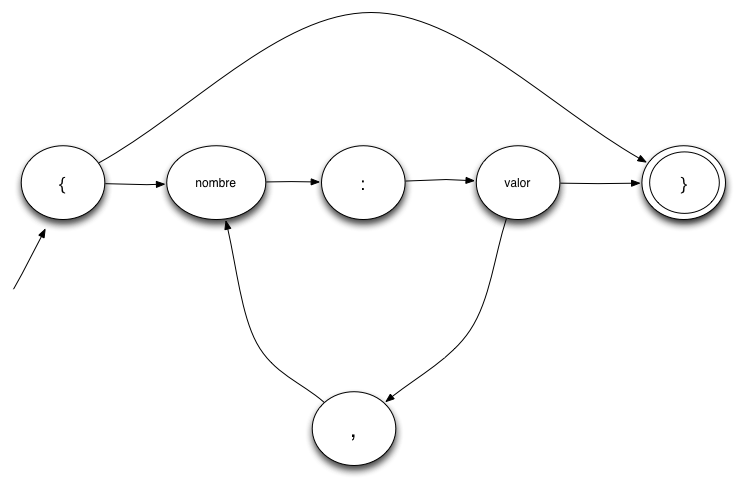
\includegraphics[scale=0.50]{images/capitulo3/afd1.png}
\caption{\textbf{Objeto:} conjunto desordenado de pares nombre/valor.}
\label{objeto}
\end{figure}

Un arreglo es una colección de valores, que comienza con [(corchete izquierdo) y termina con ] (corchete derecho). Los valores son separados por , (coma). Lo anterior, se aprecia en la máquina de estado finito en la Figura 6.\\

\begin{figure}[H]
\centering
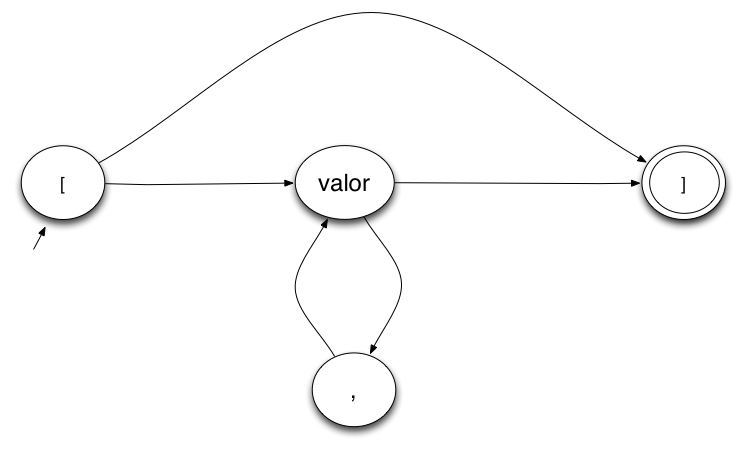
\includegraphics[scale=0.50]{images/capitulo3/afd2.png}
\caption{\textbf{Arreglo:} colección de valores separados por ',' (coma).}
\label{arreglo}
\end{figure}

Un valor puede ser una cadena de caracteres, o número, u objeto, o arreglo, o true, o false, o null.  Lo anterior, se aprecia en la máquina de estado finito en la Figura 7.\\

\begin{figure}[H]
\centering
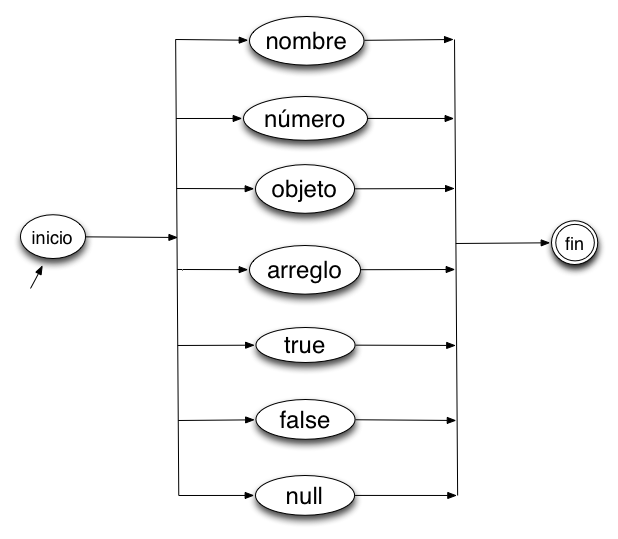
\includegraphics[scale=0.50]{images/capitulo3/afd3.png}
\caption{\textbf{Valor:} cadena de caracteres, o número, u objeto, o arreglo, o true, o false, o null.}
\label{valor}
\end{figure}

\subsubsection{Base de datos}

Para almacenar los datos proporcionados por la aplicación móvil y el módulo web,  se utilizará el sistema de gestión de bases de datos relacionales MySQL. En este apartado no se ahondará  sobre este sistema pues fue descrito en el capítulo anterior, en el punto 2.1.5.\\

\subsubsection{Librerías utilizadas}

La única librería incluída en el proyecto y que hace posible la comunicación entre la aplicación móvil y GCM: enviar y recibir notificaciones es la librería de GoogleCloudMessaging. Ésta debe ser incluida en el proyecto en \textit{Android Studio} para utilizar sus clases desde nuestra aplicación.\\

\subsubsection{Patrón MVC}

El acrónimo MVC corresponde a: \textbf{Modelo} - \textbf{Vista} - \textbf{Controlador}. Éste es un patrón de arquitectura de \textit{software} donde en una aplicación separa los datos y la lógica del negocio de la interfaz de usuario y el módulo que se encarga de gestionar los eventos y comunicaciones. Por lo anterior, MVC propone que se construyan tres componentes diferentes: el modelo, la vista y el controlador y que al final se relacionarán para tener como resultado una aplicación, en el caso del proyecto una aplicación móvil.\\ 

Para entender la Figura 8, se explicará brevemente de qué se trata cada uno de los componentes de este modelo.\\

\begin{figure}[H]
\centering
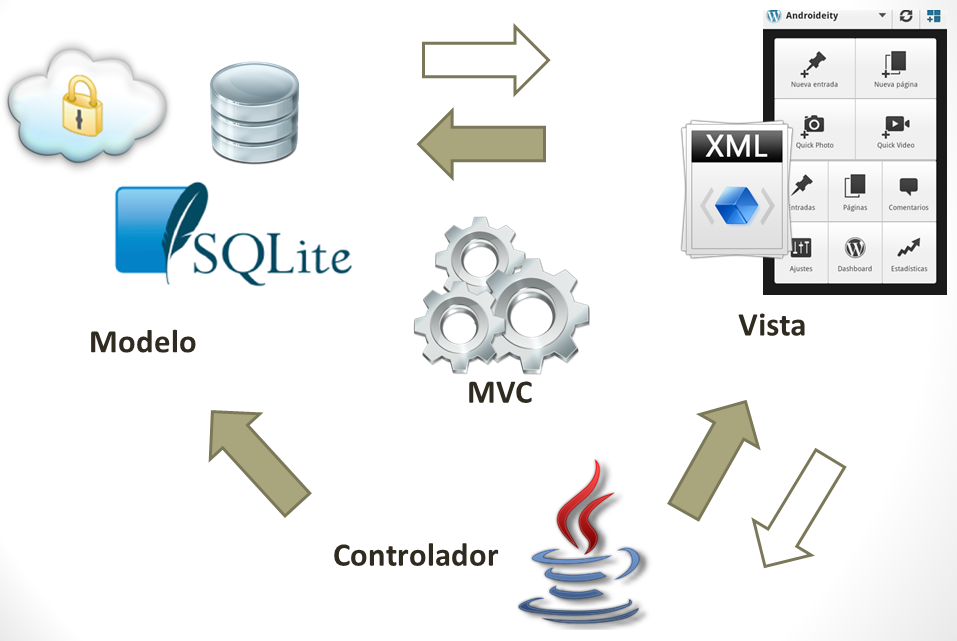
\includegraphics[scale=0.50]{images/capitulo3/mvc.png}
\caption{Patrón MVC.\cite{And12}}
\label{valor}
\end{figure}

\begin{enumerate}
\item \textbf{Modelo:} Básicamente el modelo corresponde a qué base de datos o servicios web se utilizará para almacenar la información. El modelo a elegir depende directamente de las necesidades de información que tenga la aplicación que se desarrollará.
\item \textbf{Vista:} La vista no es mas que la interfaz con la que va a interactuar el usuario. En \textit{Android}, las interfaces se construyen en XML, y es a través de éstas que se presentan los datos a los usuarios.
\item \textbf{Controlador:} Son las clases que contienen el código y permiten darle vida a las interfaces construidas permitiendo desplegar y consumir información de/para el usuario. En un proyecto \textit{Android} los controladores corresponden a las clases programadas en lenguaje JAVA y son el núcleo de la aplicación.
\end{enumerate}

\subsection{Arquitectura del sistema}

En los puntos anteriores se ha descrito lo concerniente a cómo y qué tecnologías se utilizarán para dar solución al problema expuesto. Por último, para dar sentido a lo antes planteado en los tópicos anteriores, es factible definir una arquitectura para el sistema. Ver Figura 9. La arquitectura planteada, se compone de un servidor central provisto de diversos servicios, \textit{smartphones} que se comunicarán con el sistema, una base de datos para almacenar la información, un monitor que mostrará el turno que está siendo atendido, el servicio de GCM por el cual circulan las notificaciones y un módulo web de reportes. 

\begin{figure}[H]
\centering
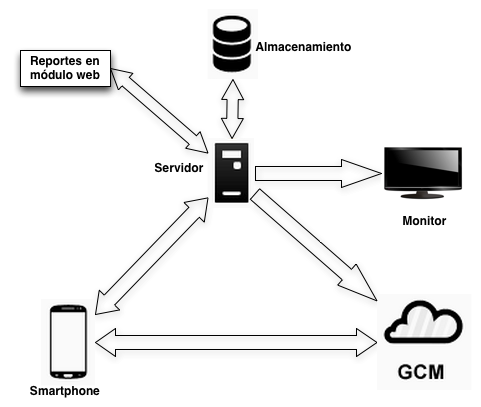
\includegraphics[scale=0.70]{images/capitulo3/arquitectura.png}
\caption{Arquitectura del sistema.}
\label{arquitectura}
\end{figure}